\documentclass[twoside]{book}

% Packages required by doxygen
\usepackage{fixltx2e}
\usepackage{calc}
\usepackage{doxygen}
\usepackage[export]{adjustbox} % also loads graphicx
\usepackage{graphicx}
\usepackage[utf8]{inputenc}
\usepackage{makeidx}
\usepackage{multicol}
\usepackage{multirow}
\PassOptionsToPackage{warn}{textcomp}
\usepackage{textcomp}
\usepackage[nointegrals]{wasysym}
\usepackage[table]{xcolor}

% Font selection
\usepackage[T1]{fontenc}
\usepackage[scaled=.90]{helvet}
\usepackage{courier}
\usepackage{amssymb}
\usepackage{sectsty}
\renewcommand{\familydefault}{\sfdefault}
\allsectionsfont{%
  \fontseries{bc}\selectfont%
  \color{darkgray}%
}
\renewcommand{\DoxyLabelFont}{%
  \fontseries{bc}\selectfont%
  \color{darkgray}%
}
\newcommand{\+}{\discretionary{\mbox{\scriptsize$\hookleftarrow$}}{}{}}

% Page & text layout
\usepackage{geometry}
\geometry{%
  a4paper,%
  top=2.5cm,%
  bottom=2.5cm,%
  left=2.5cm,%
  right=2.5cm%
}
\tolerance=750
\hfuzz=15pt
\hbadness=750
\setlength{\emergencystretch}{15pt}
\setlength{\parindent}{0cm}
\setlength{\parskip}{3ex plus 2ex minus 2ex}
\makeatletter
\renewcommand{\paragraph}{%
  \@startsection{paragraph}{4}{0ex}{-1.0ex}{1.0ex}{%
    \normalfont\normalsize\bfseries\SS@parafont%
  }%
}
\renewcommand{\subparagraph}{%
  \@startsection{subparagraph}{5}{0ex}{-1.0ex}{1.0ex}{%
    \normalfont\normalsize\bfseries\SS@subparafont%
  }%
}
\makeatother

% Headers & footers
\usepackage{fancyhdr}
\pagestyle{fancyplain}
\fancyhead[LE]{\fancyplain{}{\bfseries\thepage}}
\fancyhead[CE]{\fancyplain{}{}}
\fancyhead[RE]{\fancyplain{}{\bfseries\leftmark}}
\fancyhead[LO]{\fancyplain{}{\bfseries\rightmark}}
\fancyhead[CO]{\fancyplain{}{}}
\fancyhead[RO]{\fancyplain{}{\bfseries\thepage}}
\fancyfoot[LE]{\fancyplain{}{}}
\fancyfoot[CE]{\fancyplain{}{}}
\fancyfoot[RE]{\fancyplain{}{\bfseries\scriptsize Generated by Doxygen }}
\fancyfoot[LO]{\fancyplain{}{\bfseries\scriptsize Generated by Doxygen }}
\fancyfoot[CO]{\fancyplain{}{}}
\fancyfoot[RO]{\fancyplain{}{}}
\renewcommand{\footrulewidth}{0.4pt}
\renewcommand{\chaptermark}[1]{%
  \markboth{#1}{}%
}
\renewcommand{\sectionmark}[1]{%
  \markright{\thesection\ #1}%
}

% Indices & bibliography
\usepackage{natbib}
\usepackage[titles]{tocloft}
\setcounter{tocdepth}{3}
\setcounter{secnumdepth}{5}
\makeindex

% Hyperlinks (required, but should be loaded last)
\usepackage{ifpdf}
\ifpdf
  \usepackage[pdftex,pagebackref=true]{hyperref}
\else
  \usepackage[ps2pdf,pagebackref=true]{hyperref}
\fi
\hypersetup{%
  colorlinks=true,%
  linkcolor=blue,%
  citecolor=blue,%
  unicode%
}

% Custom commands
\newcommand{\clearemptydoublepage}{%
  \newpage{\pagestyle{empty}\cleardoublepage}%
}

\usepackage{caption}
\captionsetup{labelsep=space,justification=centering,font={bf},singlelinecheck=off,skip=4pt,position=top}

%===== C O N T E N T S =====

\begin{document}

% Titlepage & ToC
\hypersetup{pageanchor=false,
             bookmarksnumbered=true,
             pdfencoding=unicode
            }
\pagenumbering{roman}
\begin{titlepage}
\vspace*{7cm}
\begin{center}%
{\Large uio }\\
\vspace*{1cm}
{\large Generated by Doxygen 1.8.11}\\
\end{center}
\end{titlepage}
\clearemptydoublepage
\tableofcontents
\clearemptydoublepage
\pagenumbering{arabic}
\hypersetup{pageanchor=true}

%--- Begin generated contents ---
\chapter{Main Page}
\label{index}\hypertarget{index}{}\hypertarget{index_DESCRIPTION}{}\section{D\+E\+S\+C\+R\+I\+P\+T\+I\+ON}\label{index_DESCRIPTION}
\begin{DoxyParagraph}{}
uio is a portable I/O abstraction layer for low-\/performance systems such as microcontrollers.
\end{DoxyParagraph}
\hypertarget{index_LICENSE}{}\section{L\+I\+C\+E\+N\+SE}\label{index_LICENSE}
\begin{DoxyParagraph}{}
M\+IT License
\end{DoxyParagraph}
\begin{DoxyParagraph}{}
Copyright (c) 2018 Liam Bindle
\end{DoxyParagraph}
\begin{DoxyParagraph}{}
Permission is hereby granted, free of charge, to any person obtaining a copy of this software and associated documentation files (the \char`\"{}\+Software\char`\"{}), to deal in the Software without restriction, including without limitation the rights to use, copy, modify, merge, publish, distribute, sublicense, and/or sell copies of the Software, and to permit persons to whom the Software is furnished to do so, subject to the following conditions\+:
\end{DoxyParagraph}
\begin{DoxyParagraph}{}
The above copyright notice and this permission notice shall be included in all copies or substantial portions of the Software.
\end{DoxyParagraph}
\begin{DoxyParagraph}{}
T\+HE S\+O\+F\+T\+W\+A\+RE IS P\+R\+O\+V\+I\+D\+ED \char`\"{}\+A\+S I\+S\char`\"{}, W\+I\+T\+H\+O\+UT W\+A\+R\+R\+A\+N\+TY OF A\+NY K\+I\+ND, E\+X\+P\+R\+E\+SS OR I\+M\+P\+L\+I\+ED, I\+N\+C\+L\+U\+D\+I\+NG B\+UT N\+OT L\+I\+M\+I\+T\+ED TO T\+HE W\+A\+R\+R\+A\+N\+T\+I\+ES OF M\+E\+R\+C\+H\+A\+N\+T\+A\+B\+I\+L\+I\+TY, F\+I\+T\+N\+E\+SS F\+OR A P\+A\+R\+T\+I\+C\+U\+L\+AR P\+U\+R\+P\+O\+SE A\+ND N\+O\+N\+I\+N\+F\+R\+I\+N\+G\+E\+M\+E\+NT. IN NO E\+V\+E\+NT S\+H\+A\+LL T\+HE A\+U\+T\+H\+O\+RS OR C\+O\+P\+Y\+R\+I\+G\+HT H\+O\+L\+D\+E\+RS BE L\+I\+A\+B\+LE F\+OR A\+NY C\+L\+A\+IM, D\+A\+M\+A\+G\+ES OR O\+T\+H\+ER L\+I\+A\+B\+I\+L\+I\+TY, W\+H\+E\+T\+H\+ER IN AN A\+C\+T\+I\+ON OF C\+O\+N\+T\+R\+A\+CT, T\+O\+RT OR O\+T\+H\+E\+R\+W\+I\+SE, A\+R\+I\+S\+I\+NG F\+R\+OM, O\+UT OF OR IN C\+O\+N\+N\+E\+C\+T\+I\+ON W\+I\+TH T\+HE S\+O\+F\+T\+W\+A\+RE OR T\+HE U\+SE OR O\+T\+H\+ER D\+E\+A\+L\+I\+N\+GS IN T\+HE S\+O\+F\+T\+W\+A\+RE. 
\end{DoxyParagraph}

\chapter{Hierarchical Index}
\section{Class Hierarchy}
This inheritance list is sorted roughly, but not completely, alphabetically\+:\begin{DoxyCompactList}
\item \contentsline{section}{uio\+:\+:stream\+\_\+base}{\pageref{classuio_1_1stream__base}}{}
\begin{DoxyCompactList}
\item \contentsline{section}{uio\+:\+:istream}{\pageref{classuio_1_1istream}}{}
\begin{DoxyCompactList}
\item \contentsline{section}{uio\+:\+:iostream}{\pageref{classuio_1_1iostream}}{}
\end{DoxyCompactList}
\item \contentsline{section}{uio\+:\+:ostream}{\pageref{classuio_1_1ostream}}{}
\begin{DoxyCompactList}
\item \contentsline{section}{uio\+:\+:iostream}{\pageref{classuio_1_1iostream}}{}
\end{DoxyCompactList}
\item \contentsline{section}{uio\+:\+:streambuf}{\pageref{classuio_1_1streambuf}}{}
\end{DoxyCompactList}
\item \contentsline{section}{uio\+:\+:streamerr}{\pageref{classuio_1_1streamerr}}{}
\end{DoxyCompactList}

\chapter{Class Index}
\section{Class List}
Here are the classes, structs, unions and interfaces with brief descriptions\+:\begin{DoxyCompactList}
\item\contentsline{section}{\hyperlink{classuio_1_1iostream}{uio\+::iostream} \\*An input and output data stream }{\pageref{classuio_1_1iostream}}{}
\item\contentsline{section}{\hyperlink{classuio_1_1istream}{uio\+::istream} \\*An input data object }{\pageref{classuio_1_1istream}}{}
\item\contentsline{section}{\hyperlink{classuio_1_1ostream}{uio\+::ostream} \\*An output data object }{\pageref{classuio_1_1ostream}}{}
\item\contentsline{section}{\hyperlink{classuio_1_1stream__base}{uio\+::stream\+\_\+base} \\*Base class for all stream objects }{\pageref{classuio_1_1stream__base}}{}
\item\contentsline{section}{\hyperlink{classuio_1_1streambuf}{uio\+::streambuf} \\*A simple byte-\/buffer }{\pageref{classuio_1_1streambuf}}{}
\item\contentsline{section}{\hyperlink{classuio_1_1streamerr}{uio\+::streamerr} \\*Class to manage stream errors }{\pageref{classuio_1_1streamerr}}{}
\end{DoxyCompactList}

\chapter{File Index}
\section{File List}
Here is a list of all documented files with brief descriptions\+:\begin{DoxyCompactList}
\item\contentsline{section}{\hyperlink{uio_8hpp}{uio.\+hpp} }{\pageref{uio_8hpp}}{}
\end{DoxyCompactList}

\chapter{Class Documentation}
\hypertarget{classuio_1_1iostream}{}\section{uio\+:\+:iostream Class Reference}
\label{classuio_1_1iostream}\index{uio\+::iostream@{uio\+::iostream}}


An input and output data stream.  




{\ttfamily \#include $<$uio.\+hpp$>$}



Inheritance diagram for uio\+:\+:iostream\+:\nopagebreak
\begin{figure}[H]
\begin{center}
\leavevmode
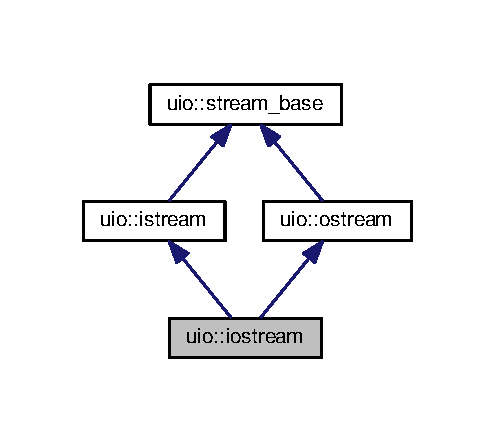
\includegraphics[width=238pt]{classuio_1_1iostream__inherit__graph}
\end{center}
\end{figure}
\subsection*{Additional Inherited Members}


\subsection{Detailed Description}
An input and output data stream. 

The documentation for this class was generated from the following file\+:\begin{DoxyCompactItemize}
\item 
\hyperlink{uio_8hpp}{uio.\+hpp}\end{DoxyCompactItemize}

\hypertarget{classuio_1_1istream}{}\section{uio\+:\+:istream Class Reference}
\label{classuio_1_1istream}\index{uio\+::istream@{uio\+::istream}}


An input data object.  




{\ttfamily \#include $<$uio.\+hpp$>$}



Inheritance diagram for uio\+:\+:istream\+:\nopagebreak
\begin{figure}[H]
\begin{center}
\leavevmode
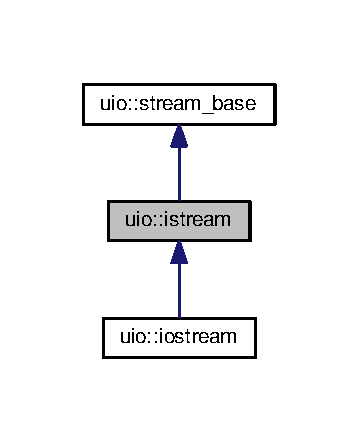
\includegraphics[width=172pt]{classuio_1_1istream__inherit__graph}
\end{center}
\end{figure}
\subsection*{Public Member Functions}
\begin{DoxyCompactItemize}
\item 
virtual \hyperlink{classuio_1_1istream}{istream} \& \hyperlink{classuio_1_1istream_ac98975f13fe7d94de24ce9e9073daaae}{operator$>$$>$} (char $\ast$s)
\begin{DoxyCompactList}\small\item\em Convenience function for writing input data to {\ttfamily string}. \end{DoxyCompactList}\item 
virtual size\+\_\+t \hyperlink{classuio_1_1istream_ac351e3f745e1e10d1d4f999ba097222a}{gcount} ()
\begin{DoxyCompactList}\small\item\em Returns the number of bytes that can be gotten using \hyperlink{classuio_1_1istream_a2cd3af4694dd6680a16221a8e77a344b}{get}. \end{DoxyCompactList}\item 
virtual size\+\_\+t \hyperlink{classuio_1_1istream_a2cd3af4694dd6680a16221a8e77a344b}{get} (char $\ast$buf)
\begin{DoxyCompactList}\small\item\em Get the next byte from the input data stream. \end{DoxyCompactList}\item 
virtual size\+\_\+t \hyperlink{classuio_1_1istream_a12e8ae6afd488b62e216333dbb0935cc}{get} (char $\ast$buf, size\+\_\+t buflen)
\begin{DoxyCompactList}\small\item\em Copy up to {\itshape buflen} bytes to {\itshape buf}. \end{DoxyCompactList}\item 
virtual \hyperlink{classuio_1_1istream}{istream} \& \hyperlink{classuio_1_1istream_a06381289f359f89adb4f26a32b128139}{sync} ()=0
\begin{DoxyCompactList}\small\item\em Pure virtual function to synchronize (update) input data stream. \end{DoxyCompactList}\end{DoxyCompactItemize}
\subsection*{Public Attributes}
\begin{DoxyCompactItemize}
\item 
\hyperlink{classuio_1_1streamerr}{streamerr} \hyperlink{classuio_1_1istream_a31e0fa22aa929184ac32b0cbff9c545d}{\+\_\+ierror}\hypertarget{classuio_1_1istream_a31e0fa22aa929184ac32b0cbff9c545d}{}\label{classuio_1_1istream_a31e0fa22aa929184ac32b0cbff9c545d}

\begin{DoxyCompactList}\small\item\em Input stream \hyperlink{classuio_1_1streamerr}{streamerr}. \end{DoxyCompactList}\end{DoxyCompactItemize}
\subsection*{Protected Attributes}
\begin{DoxyCompactItemize}
\item 
\hyperlink{classuio_1_1streambuf}{streambuf} \hyperlink{classuio_1_1istream_a9291e43c0a3cbb43fc0c497ba332056a}{\+\_\+ibuf}\hypertarget{classuio_1_1istream_a9291e43c0a3cbb43fc0c497ba332056a}{}\label{classuio_1_1istream_a9291e43c0a3cbb43fc0c497ba332056a}

\begin{DoxyCompactList}\small\item\em Input data \hyperlink{classuio_1_1streambuf}{streambuf}. \end{DoxyCompactList}\end{DoxyCompactItemize}


\subsection{Detailed Description}
An input data object. 

\hyperlink{classuio_1_1istream}{istream} is an object that supports the following operations\+: \begin{DoxyItemize}
\item \hyperlink{classuio_1_1istream_ac351e3f745e1e10d1d4f999ba097222a}{gcount} \item \hyperlink{classuio_1_1istream_a2cd3af4694dd6680a16221a8e77a344b}{get} \item \hyperlink{classuio_1_1istream_a06381289f359f89adb4f26a32b128139}{sync}\end{DoxyItemize}
\begin{DoxyNote}{Note}
Input data might not be automatically synchronized. Users should call \hyperlink{classuio_1_1istream_a06381289f359f89adb4f26a32b128139}{sync} before \hyperlink{classuio_1_1istream_a2cd3af4694dd6680a16221a8e77a344b}{get}. 
\end{DoxyNote}


\subsection{Member Function Documentation}
\index{uio\+::istream@{uio\+::istream}!gcount@{gcount}}
\index{gcount@{gcount}!uio\+::istream@{uio\+::istream}}
\subsubsection[{\texorpdfstring{gcount()}{gcount()}}]{\setlength{\rightskip}{0pt plus 5cm}virtual size\+\_\+t uio\+::istream\+::gcount (
\begin{DoxyParamCaption}
{}
\end{DoxyParamCaption}
)\hspace{0.3cm}{\ttfamily [inline]}, {\ttfamily [virtual]}}\hypertarget{classuio_1_1istream_ac351e3f745e1e10d1d4f999ba097222a}{}\label{classuio_1_1istream_ac351e3f745e1e10d1d4f999ba097222a}


Returns the number of bytes that can be gotten using \hyperlink{classuio_1_1istream_a2cd3af4694dd6680a16221a8e77a344b}{get}. 

\begin{DoxySeeAlso}{See also}
\hyperlink{classuio_1_1istream_a2cd3af4694dd6680a16221a8e77a344b}{get}
\end{DoxySeeAlso}
\begin{DoxyReturn}{Returns}
The number of bytes that can be read. 
\end{DoxyReturn}
\index{uio\+::istream@{uio\+::istream}!get@{get}}
\index{get@{get}!uio\+::istream@{uio\+::istream}}
\subsubsection[{\texorpdfstring{get(char $\ast$buf)}{get(char *buf)}}]{\setlength{\rightskip}{0pt plus 5cm}virtual size\+\_\+t uio\+::istream\+::get (
\begin{DoxyParamCaption}
\item[{char $\ast$}]{buf}
\end{DoxyParamCaption}
)\hspace{0.3cm}{\ttfamily [inline]}, {\ttfamily [virtual]}}\hypertarget{classuio_1_1istream_a2cd3af4694dd6680a16221a8e77a344b}{}\label{classuio_1_1istream_a2cd3af4694dd6680a16221a8e77a344b}


Get the next byte from the input data stream. 


\begin{DoxyParams}[1]{Parameters}
\mbox{\tt out}  & {\em buf} & Address to copy the next input data byte to.\\
\hline
\end{DoxyParams}
\begin{DoxyReturn}{Returns}
1 if the next byte was copied, 0 otherwise (i.\+e. no more bytes to be read). 
\end{DoxyReturn}
\index{uio\+::istream@{uio\+::istream}!get@{get}}
\index{get@{get}!uio\+::istream@{uio\+::istream}}
\subsubsection[{\texorpdfstring{get(char $\ast$buf, size\+\_\+t buflen)}{get(char *buf, size_t buflen)}}]{\setlength{\rightskip}{0pt plus 5cm}virtual size\+\_\+t uio\+::istream\+::get (
\begin{DoxyParamCaption}
\item[{char $\ast$}]{buf, }
\item[{size\+\_\+t}]{buflen}
\end{DoxyParamCaption}
)\hspace{0.3cm}{\ttfamily [inline]}, {\ttfamily [virtual]}}\hypertarget{classuio_1_1istream_a12e8ae6afd488b62e216333dbb0935cc}{}\label{classuio_1_1istream_a12e8ae6afd488b62e216333dbb0935cc}


Copy up to {\itshape buflen} bytes to {\itshape buf}. 

If {\itshape buflen} is greater than the number of bytes that can be gotten (\hyperlink{classuio_1_1istream_ac351e3f745e1e10d1d4f999ba097222a}{gcount}), then only \hyperlink{classuio_1_1istream_ac351e3f745e1e10d1d4f999ba097222a}{gcount} bytes will be copied to {\itshape buf}.


\begin{DoxyParams}[1]{Parameters}
\mbox{\tt out}  & {\em buf} & First address to start copying bytes to. \\
\hline
\mbox{\tt in}  & {\em buflen} & Maximum number of bytes to be copied to {\itshape buf}.\\
\hline
\end{DoxyParams}
\begin{DoxyReturn}{Returns}
Number of bytes copied to {\itshape buf}. 
\end{DoxyReturn}
\index{uio\+::istream@{uio\+::istream}!operator$>$$>$@{operator$>$$>$}}
\index{operator$>$$>$@{operator$>$$>$}!uio\+::istream@{uio\+::istream}}
\subsubsection[{\texorpdfstring{operator$>$$>$(char $\ast$s)}{operator>>(char *s)}}]{\setlength{\rightskip}{0pt plus 5cm}virtual {\bf istream}\& uio\+::istream\+::operator$>$$>$ (
\begin{DoxyParamCaption}
\item[{char $\ast$}]{s}
\end{DoxyParamCaption}
)\hspace{0.3cm}{\ttfamily [inline]}, {\ttfamily [virtual]}}\hypertarget{classuio_1_1istream_ac98975f13fe7d94de24ce9e9073daaae}{}\label{classuio_1_1istream_ac98975f13fe7d94de24ce9e9073daaae}


Convenience function for writing input data to {\ttfamily string}. 

\hyperlink{classuio_1_1istream_ac351e3f745e1e10d1d4f999ba097222a}{gcount} characters are copied to {\itshape s}, as well as a null character. This means that \hyperlink{classuio_1_1istream_ac351e3f745e1e10d1d4f999ba097222a}{gcount} plus 1 bytes are copied to {\itshape s}.

\begin{DoxyAttention}{Attention}
This function has no safe-\/guards to check that {\itshape s} is large enough to store the entire input data streams contents.
\end{DoxyAttention}

\begin{DoxyParams}[1]{Parameters}
\mbox{\tt out}  & {\em s} & First address of character array.\\
\hline
\end{DoxyParams}
\begin{DoxyReturn}{Returns}
{\ttfamily $\ast$this} 
\end{DoxyReturn}
\index{uio\+::istream@{uio\+::istream}!sync@{sync}}
\index{sync@{sync}!uio\+::istream@{uio\+::istream}}
\subsubsection[{\texorpdfstring{sync()=0}{sync()=0}}]{\setlength{\rightskip}{0pt plus 5cm}virtual {\bf istream}\& uio\+::istream\+::sync (
\begin{DoxyParamCaption}
{}
\end{DoxyParamCaption}
)\hspace{0.3cm}{\ttfamily [pure virtual]}}\hypertarget{classuio_1_1istream_a06381289f359f89adb4f26a32b128139}{}\label{classuio_1_1istream_a06381289f359f89adb4f26a32b128139}


Pure virtual function to synchronize (update) input data stream. 

This function updates the internal buffers (i.\+e. does whatever needs to happend to bring the internal buffers up to date).

\begin{DoxyNote}{Note}
It might be necessary to call this function before \hyperlink{classuio_1_1istream_a2cd3af4694dd6680a16221a8e77a344b}{get}.
\end{DoxyNote}
\begin{DoxyReturn}{Returns}
{\ttfamily $\ast$this} 
\end{DoxyReturn}


The documentation for this class was generated from the following file\+:\begin{DoxyCompactItemize}
\item 
\hyperlink{uio_8hpp}{uio.\+hpp}\end{DoxyCompactItemize}

\hypertarget{classuio_1_1ostream}{}\section{uio\+:\+:ostream Class Reference}
\label{classuio_1_1ostream}\index{uio\+::ostream@{uio\+::ostream}}


An output data object.  




{\ttfamily \#include $<$uio.\+hpp$>$}



Inheritance diagram for uio\+:\+:ostream\+:\nopagebreak
\begin{figure}[H]
\begin{center}
\leavevmode
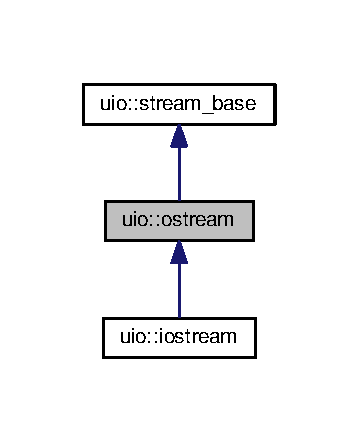
\includegraphics[width=172pt]{classuio_1_1ostream__inherit__graph}
\end{center}
\end{figure}
\subsection*{Public Member Functions}
\begin{DoxyCompactItemize}
\item 
virtual \hyperlink{classuio_1_1ostream}{ostream} \& \hyperlink{classuio_1_1ostream_a9997cc4d79bc6019fe554efe188f923e}{operator$<$$<$} (const char $\ast$s)
\begin{DoxyCompactList}\small\item\em Convenience function for writing output data from a {\ttfamily string}. \end{DoxyCompactList}\item 
virtual \hyperlink{classuio_1_1ostream}{ostream} \& \hyperlink{classuio_1_1ostream_aeffd1b2ee0a79a6728840811c7ad1770}{put} (char c)
\begin{DoxyCompactList}\small\item\em Write byte to output data stream. \end{DoxyCompactList}\item 
virtual \hyperlink{classuio_1_1ostream}{ostream} \& \hyperlink{classuio_1_1ostream_a4da5a561a3547e3a3793618860182354}{write} (const char $\ast$s, size\+\_\+t n)
\begin{DoxyCompactList}\small\item\em Write {\itshape n} bytes from {\itshape s} to the output data stream. \end{DoxyCompactList}\item 
virtual \hyperlink{classuio_1_1ostream}{ostream} \& \hyperlink{classuio_1_1ostream_a8c398c36b7619aa7cf32da064bce64d3}{flush} ()=0
\begin{DoxyCompactList}\small\item\em A pure virtual function to flush buffered data to output data stream. \end{DoxyCompactList}\end{DoxyCompactItemize}
\subsection*{Public Attributes}
\begin{DoxyCompactItemize}
\item 
\hyperlink{classuio_1_1streamerr}{streamerr} \hyperlink{classuio_1_1ostream_aaba80028bfff5f9d12f40789db0c8d58}{\+\_\+oerror}\hypertarget{classuio_1_1ostream_aaba80028bfff5f9d12f40789db0c8d58}{}\label{classuio_1_1ostream_aaba80028bfff5f9d12f40789db0c8d58}

\begin{DoxyCompactList}\small\item\em Output stream \hyperlink{classuio_1_1streamerr}{streamerr}. \end{DoxyCompactList}\end{DoxyCompactItemize}
\subsection*{Protected Attributes}
\begin{DoxyCompactItemize}
\item 
\hyperlink{classuio_1_1streambuf}{streambuf} \hyperlink{classuio_1_1ostream_a9f8d3fae9009a4d06bfc12af161a3ca2}{\+\_\+obuf}\hypertarget{classuio_1_1ostream_a9f8d3fae9009a4d06bfc12af161a3ca2}{}\label{classuio_1_1ostream_a9f8d3fae9009a4d06bfc12af161a3ca2}

\begin{DoxyCompactList}\small\item\em Output stream \hyperlink{classuio_1_1streambuf}{streambuf}. \end{DoxyCompactList}\end{DoxyCompactItemize}


\subsection{Detailed Description}
An output data object. 

\hyperlink{classuio_1_1ostream}{ostream} is an object that supports the following operations\+: \begin{DoxyItemize}
\item \hyperlink{classuio_1_1ostream_aeffd1b2ee0a79a6728840811c7ad1770}{put} \item \hyperlink{classuio_1_1ostream_a8c398c36b7619aa7cf32da064bce64d3}{flush}\end{DoxyItemize}
\begin{DoxyNote}{Note}
Output data might not be automatically flushed. Users should call \hyperlink{classuio_1_1ostream_a8c398c36b7619aa7cf32da064bce64d3}{flush} when they want the internal buffers to be written out. 
\end{DoxyNote}


\subsection{Member Function Documentation}
\index{uio\+::ostream@{uio\+::ostream}!flush@{flush}}
\index{flush@{flush}!uio\+::ostream@{uio\+::ostream}}
\subsubsection[{\texorpdfstring{flush()=0}{flush()=0}}]{\setlength{\rightskip}{0pt plus 5cm}virtual {\bf ostream}\& uio\+::ostream\+::flush (
\begin{DoxyParamCaption}
{}
\end{DoxyParamCaption}
)\hspace{0.3cm}{\ttfamily [pure virtual]}}\hypertarget{classuio_1_1ostream_a8c398c36b7619aa7cf32da064bce64d3}{}\label{classuio_1_1ostream_a8c398c36b7619aa7cf32da064bce64d3}


A pure virtual function to flush buffered data to output data stream. 

This function does whatever is necessary to output the buffered data.

\begin{DoxyReturn}{Returns}
{\ttfamily $\ast$this} 
\end{DoxyReturn}
\index{uio\+::ostream@{uio\+::ostream}!operator$<$$<$@{operator$<$$<$}}
\index{operator$<$$<$@{operator$<$$<$}!uio\+::ostream@{uio\+::ostream}}
\subsubsection[{\texorpdfstring{operator$<$$<$(const char $\ast$s)}{operator<<(const char *s)}}]{\setlength{\rightskip}{0pt plus 5cm}virtual {\bf ostream}\& uio\+::ostream\+::operator$<$$<$ (
\begin{DoxyParamCaption}
\item[{const char $\ast$}]{s}
\end{DoxyParamCaption}
)\hspace{0.3cm}{\ttfamily [inline]}, {\ttfamily [virtual]}}\hypertarget{classuio_1_1ostream_a9997cc4d79bc6019fe554efe188f923e}{}\label{classuio_1_1ostream_a9997cc4d79bc6019fe554efe188f923e}


Convenience function for writing output data from a {\ttfamily string}. 

\begin{DoxyNote}{Note}
The null character at the end of {\itshape s} is {\itshape not} copied to the buffer.

{\ttfamily \+\_\+oerror.\+\_\+flags.\+overflow} is set if there is not enough space in the output buffer.
\end{DoxyNote}

\begin{DoxyParams}[1]{Parameters}
\mbox{\tt out}  & {\em s} & Character array to write to output stream.\\
\hline
\end{DoxyParams}
\begin{DoxyReturn}{Returns}
{\ttfamily $\ast$this} 
\end{DoxyReturn}
\index{uio\+::ostream@{uio\+::ostream}!put@{put}}
\index{put@{put}!uio\+::ostream@{uio\+::ostream}}
\subsubsection[{\texorpdfstring{put(char c)}{put(char c)}}]{\setlength{\rightskip}{0pt plus 5cm}virtual {\bf ostream}\& uio\+::ostream\+::put (
\begin{DoxyParamCaption}
\item[{char}]{c}
\end{DoxyParamCaption}
)\hspace{0.3cm}{\ttfamily [inline]}, {\ttfamily [virtual]}}\hypertarget{classuio_1_1ostream_aeffd1b2ee0a79a6728840811c7ad1770}{}\label{classuio_1_1ostream_aeffd1b2ee0a79a6728840811c7ad1770}


Write byte to output data stream. 


\begin{DoxyParams}[1]{Parameters}
\mbox{\tt in}  & {\em c} & The byte\textquotesingle{}s value.\\
\hline
\end{DoxyParams}
\begin{DoxyNote}{Note}
{\ttfamily \+\_\+oerror.\+\_\+flags.\+overflow} is set if there is not enough space in the output buffer.
\end{DoxyNote}
\begin{DoxyReturn}{Returns}
{\ttfamily $\ast$this} 
\end{DoxyReturn}
\index{uio\+::ostream@{uio\+::ostream}!write@{write}}
\index{write@{write}!uio\+::ostream@{uio\+::ostream}}
\subsubsection[{\texorpdfstring{write(const char $\ast$s, size\+\_\+t n)}{write(const char *s, size_t n)}}]{\setlength{\rightskip}{0pt plus 5cm}virtual {\bf ostream}\& uio\+::ostream\+::write (
\begin{DoxyParamCaption}
\item[{const char $\ast$}]{s, }
\item[{size\+\_\+t}]{n}
\end{DoxyParamCaption}
)\hspace{0.3cm}{\ttfamily [inline]}, {\ttfamily [virtual]}}\hypertarget{classuio_1_1ostream_a4da5a561a3547e3a3793618860182354}{}\label{classuio_1_1ostream_a4da5a561a3547e3a3793618860182354}


Write {\itshape n} bytes from {\itshape s} to the output data stream. 


\begin{DoxyParams}[1]{Parameters}
\mbox{\tt in}  & {\em s} & The address of the first byte to be written. \\
\hline
\mbox{\tt in}  & {\em n} & The number of bytes to be written.\\
\hline
\end{DoxyParams}
\begin{DoxyNote}{Note}
{\ttfamily \+\_\+oerror.\+\_\+flags.\+overflow} is set if there is not enough space in the output buffer.
\end{DoxyNote}
\begin{DoxyReturn}{Returns}
{\ttfamily $\ast$this} 
\end{DoxyReturn}


The documentation for this class was generated from the following file\+:\begin{DoxyCompactItemize}
\item 
\hyperlink{uio_8hpp}{uio.\+hpp}\end{DoxyCompactItemize}

\hypertarget{classuio_1_1stream__base}{}\section{uio\+:\+:stream\+\_\+base Class Reference}
\label{classuio_1_1stream__base}\index{uio\+::stream\+\_\+base@{uio\+::stream\+\_\+base}}


Base class for all stream objects.  




{\ttfamily \#include $<$uio.\+hpp$>$}



Inheritance diagram for uio\+:\+:stream\+\_\+base\+:\nopagebreak
\begin{figure}[H]
\begin{center}
\leavevmode
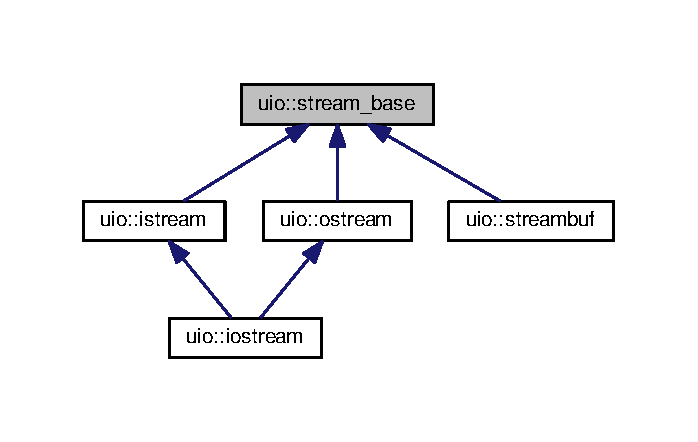
\includegraphics[width=335pt]{classuio_1_1stream__base__inherit__graph}
\end{center}
\end{figure}


\subsection{Detailed Description}
Base class for all stream objects. 

The documentation for this class was generated from the following file\+:\begin{DoxyCompactItemize}
\item 
\hyperlink{uio_8hpp}{uio.\+hpp}\end{DoxyCompactItemize}

\hypertarget{classuio_1_1streambuf}{}\section{uio\+:\+:streambuf Class Reference}
\label{classuio_1_1streambuf}\index{uio\+::streambuf@{uio\+::streambuf}}


A simple byte-\/buffer.  




{\ttfamily \#include $<$uio.\+hpp$>$}



Inheritance diagram for uio\+:\+:streambuf\+:\nopagebreak
\begin{figure}[H]
\begin{center}
\leavevmode
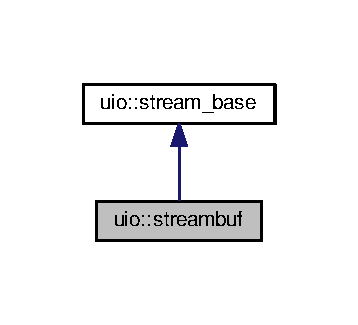
\includegraphics[width=172pt]{classuio_1_1streambuf__inherit__graph}
\end{center}
\end{figure}
\subsection*{Public Member Functions}
\begin{DoxyCompactItemize}
\item 
\hyperlink{classuio_1_1streambuf_a990efec101a2ade1c4483b604b3b975f}{streambuf} ()\hypertarget{classuio_1_1streambuf_a990efec101a2ade1c4483b604b3b975f}{}\label{classuio_1_1streambuf_a990efec101a2ade1c4483b604b3b975f}

\begin{DoxyCompactList}\small\item\em Default constructor. \end{DoxyCompactList}\item 
size\+\_\+t \hyperlink{classuio_1_1streambuf_ada2f9f2f7fb1baf6b59d03225b19c0cf}{in\+\_\+avail} () const 
\begin{DoxyCompactList}\small\item\em Get the number of bytes available to be read-\/out. \end{DoxyCompactList}\item 
size\+\_\+t \hyperlink{classuio_1_1streambuf_adaa8fa0a7ddf5869253e1cedaf252b09}{sgetc} (char $\ast$c)
\begin{DoxyCompactList}\small\item\em Get the next byte out of the buffer. \end{DoxyCompactList}\item 
size\+\_\+t \hyperlink{classuio_1_1streambuf_ab11718a2981a8842cca0fab203ad6dd9}{sgetn} (char $\ast$s, size\+\_\+t len)
\begin{DoxyCompactList}\small\item\em Copies up to {\itshape len} bytes into {\itshape s} from the buffer. \end{DoxyCompactList}\item 
size\+\_\+t \hyperlink{classuio_1_1streambuf_a6557815e43ffcab9acb8571f2dda6669}{sputc} (char c)
\begin{DoxyCompactList}\small\item\em Append {\itshape c} to the buffer. \end{DoxyCompactList}\item 
size\+\_\+t \hyperlink{classuio_1_1streambuf_ae334918cb80ba6e717ced144d5b860f7}{sputn} (const char $\ast$s, size\+\_\+t len)
\begin{DoxyCompactList}\small\item\em Copy {\itshape len} bytes from {\itshape s} to the back of the buffer. \end{DoxyCompactList}\item 
size\+\_\+t \hyperlink{classuio_1_1streambuf_a8b39ea522254c9f1c9788d2c8f1b1851}{purge} ()
\begin{DoxyCompactList}\small\item\em Clear all buffer data and error flags. \end{DoxyCompactList}\item 
\hyperlink{classuio_1_1streambuf}{streambuf} $\ast$ \hyperlink{classuio_1_1streambuf_a843b3684bd11cd1fae95a9bbc28b9794}{setbuf} (char $\ast$buf, size\+\_\+t capacity)
\begin{DoxyCompactList}\small\item\em Initialize the buffer. \end{DoxyCompactList}\item 
void $\ast$ \hyperlink{classuio_1_1streambuf_aae4696bb257ac7a41de409a01c454534}{dump} ()
\begin{DoxyCompactList}\small\item\em Get the entire contents of the buffer. \end{DoxyCompactList}\item 
size\+\_\+t \hyperlink{classuio_1_1streambuf_a5db2da142ca9bae814a73df3f794350f}{size} () const 
\begin{DoxyCompactList}\small\item\em Get the number of bytes in the buffer. \end{DoxyCompactList}\end{DoxyCompactItemize}
\subsection*{Public Attributes}
\begin{DoxyCompactItemize}
\item 
\hyperlink{classuio_1_1streamerr}{streamerr} \hyperlink{classuio_1_1streambuf_a93e2fac86ea892c0b8b33c0bc83dfd67}{\+\_\+error}\hypertarget{classuio_1_1streambuf_a93e2fac86ea892c0b8b33c0bc83dfd67}{}\label{classuio_1_1streambuf_a93e2fac86ea892c0b8b33c0bc83dfd67}

\begin{DoxyCompactList}\small\item\em The buffer\textquotesingle{}s \hyperlink{classuio_1_1streamerr}{streamerr}. \end{DoxyCompactList}\end{DoxyCompactItemize}


\subsection{Detailed Description}
A simple byte-\/buffer. 

This class implements an efficient and lightweight byte-\/buffer.

\begin{DoxyAttention}{Attention}
\hyperlink{classuio_1_1streambuf_a843b3684bd11cd1fae95a9bbc28b9794}{setbuf} {\itshape must} be called before this class can be used. 
\end{DoxyAttention}


\subsection{Member Function Documentation}
\index{uio\+::streambuf@{uio\+::streambuf}!dump@{dump}}
\index{dump@{dump}!uio\+::streambuf@{uio\+::streambuf}}
\subsubsection[{\texorpdfstring{dump()}{dump()}}]{\setlength{\rightskip}{0pt plus 5cm}void$\ast$ uio\+::streambuf\+::dump (
\begin{DoxyParamCaption}
{}
\end{DoxyParamCaption}
)\hspace{0.3cm}{\ttfamily [inline]}}\hypertarget{classuio_1_1streambuf_aae4696bb257ac7a41de409a01c454534}{}\label{classuio_1_1streambuf_aae4696bb257ac7a41de409a01c454534}


Get the entire contents of the buffer. 

Returns a pointer to the entire contents of the buffer. The contents of the buffer will be overwritten on the next call to \hyperlink{classuio_1_1streambuf_a6557815e43ffcab9acb8571f2dda6669}{sputc} or \hyperlink{classuio_1_1streambuf_ae334918cb80ba6e717ced144d5b860f7}{sputn} (this that calls to \hyperlink{classuio_1_1streambuf_a5db2da142ca9bae814a73df3f794350f}{size()} are valid until the next call to {\ttfamily sputc} or {\ttfamily sputn}).

\begin{DoxySeeAlso}{See also}
\hyperlink{classuio_1_1streambuf_a5db2da142ca9bae814a73df3f794350f}{size}
\end{DoxySeeAlso}
\begin{DoxyReturn}{Returns}
Address of the first byte in the buffer. 
\end{DoxyReturn}
\index{uio\+::streambuf@{uio\+::streambuf}!in\+\_\+avail@{in\+\_\+avail}}
\index{in\+\_\+avail@{in\+\_\+avail}!uio\+::streambuf@{uio\+::streambuf}}
\subsubsection[{\texorpdfstring{in\+\_\+avail() const }{in_avail() const }}]{\setlength{\rightskip}{0pt plus 5cm}size\+\_\+t uio\+::streambuf\+::in\+\_\+avail (
\begin{DoxyParamCaption}
{}
\end{DoxyParamCaption}
) const\hspace{0.3cm}{\ttfamily [inline]}}\hypertarget{classuio_1_1streambuf_ada2f9f2f7fb1baf6b59d03225b19c0cf}{}\label{classuio_1_1streambuf_ada2f9f2f7fb1baf6b59d03225b19c0cf}


Get the number of bytes available to be read-\/out. 

This function is equiavlent to \hyperlink{classuio_1_1streambuf_a5db2da142ca9bae814a73df3f794350f}{size} minus the internal {\ttfamily sget} cursor position.

\begin{DoxyReturn}{Returns}
Number of bytes that can be read-\/out. 
\end{DoxyReturn}
\index{uio\+::streambuf@{uio\+::streambuf}!purge@{purge}}
\index{purge@{purge}!uio\+::streambuf@{uio\+::streambuf}}
\subsubsection[{\texorpdfstring{purge()}{purge()}}]{\setlength{\rightskip}{0pt plus 5cm}size\+\_\+t uio\+::streambuf\+::purge (
\begin{DoxyParamCaption}
{}
\end{DoxyParamCaption}
)\hspace{0.3cm}{\ttfamily [inline]}}\hypertarget{classuio_1_1streambuf_a8b39ea522254c9f1c9788d2c8f1b1851}{}\label{classuio_1_1streambuf_a8b39ea522254c9f1c9788d2c8f1b1851}


Clear all buffer data and error flags. 

\begin{DoxyReturn}{Returns}
The number of bytes that were cleared from the buffer. 
\end{DoxyReturn}
\index{uio\+::streambuf@{uio\+::streambuf}!setbuf@{setbuf}}
\index{setbuf@{setbuf}!uio\+::streambuf@{uio\+::streambuf}}
\subsubsection[{\texorpdfstring{setbuf(char $\ast$buf, size\+\_\+t capacity)}{setbuf(char *buf, size_t capacity)}}]{\setlength{\rightskip}{0pt plus 5cm}{\bf streambuf}$\ast$ uio\+::streambuf\+::setbuf (
\begin{DoxyParamCaption}
\item[{char $\ast$}]{buf, }
\item[{size\+\_\+t}]{capacity}
\end{DoxyParamCaption}
)\hspace{0.3cm}{\ttfamily [inline]}}\hypertarget{classuio_1_1streambuf_a843b3684bd11cd1fae95a9bbc28b9794}{}\label{classuio_1_1streambuf_a843b3684bd11cd1fae95a9bbc28b9794}


Initialize the buffer. 

\begin{DoxyAttention}{Attention}
This function {\itshape must} be called before the buffer can be used.
\end{DoxyAttention}

\begin{DoxyParams}{Parameters}
{\em buf} & Memory allocation for this buffer. \\
\hline
{\em capacity} & Size of the buffer (i.\+e. size of {\itshape buf}).\\
\hline
\end{DoxyParams}
\begin{DoxyReturn}{Returns}
{\ttfamily this} 
\end{DoxyReturn}
\index{uio\+::streambuf@{uio\+::streambuf}!sgetc@{sgetc}}
\index{sgetc@{sgetc}!uio\+::streambuf@{uio\+::streambuf}}
\subsubsection[{\texorpdfstring{sgetc(char $\ast$c)}{sgetc(char *c)}}]{\setlength{\rightskip}{0pt plus 5cm}size\+\_\+t uio\+::streambuf\+::sgetc (
\begin{DoxyParamCaption}
\item[{char $\ast$}]{c}
\end{DoxyParamCaption}
)\hspace{0.3cm}{\ttfamily [inline]}}\hypertarget{classuio_1_1streambuf_adaa8fa0a7ddf5869253e1cedaf252b09}{}\label{classuio_1_1streambuf_adaa8fa0a7ddf5869253e1cedaf252b09}


Get the next byte out of the buffer. 


\begin{DoxyParams}[1]{Parameters}
\mbox{\tt out}  & {\em c} & Address to copy byte to.\\
\hline
\end{DoxyParams}
\begin{DoxyReturn}{Returns}
1 if a byte was copied to {\itshape c}, 0 otherwise (i.\+e. no bytes left in the buffer). 
\end{DoxyReturn}
\index{uio\+::streambuf@{uio\+::streambuf}!sgetn@{sgetn}}
\index{sgetn@{sgetn}!uio\+::streambuf@{uio\+::streambuf}}
\subsubsection[{\texorpdfstring{sgetn(char $\ast$s, size\+\_\+t len)}{sgetn(char *s, size_t len)}}]{\setlength{\rightskip}{0pt plus 5cm}size\+\_\+t uio\+::streambuf\+::sgetn (
\begin{DoxyParamCaption}
\item[{char $\ast$}]{s, }
\item[{size\+\_\+t}]{len}
\end{DoxyParamCaption}
)\hspace{0.3cm}{\ttfamily [inline]}}\hypertarget{classuio_1_1streambuf_ab11718a2981a8842cca0fab203ad6dd9}{}\label{classuio_1_1streambuf_ab11718a2981a8842cca0fab203ad6dd9}


Copies up to {\itshape len} bytes into {\itshape s} from the buffer. 

If there are fewer than {\itshape len} bytes in the buffer, \hyperlink{classuio_1_1streambuf_ada2f9f2f7fb1baf6b59d03225b19c0cf}{in\+\_\+avail()} bytes will be copied to {\itshape s}.


\begin{DoxyParams}[1]{Parameters}
\mbox{\tt out}  & {\em s} & Address to begin copying to. \\
\hline
\mbox{\tt in}  & {\em len} & Maximum number of bytes to copy.\\
\hline
\end{DoxyParams}
\begin{DoxyReturn}{Returns}
The number of bytes copied to {\itshape s}. 
\end{DoxyReturn}
\index{uio\+::streambuf@{uio\+::streambuf}!size@{size}}
\index{size@{size}!uio\+::streambuf@{uio\+::streambuf}}
\subsubsection[{\texorpdfstring{size() const }{size() const }}]{\setlength{\rightskip}{0pt plus 5cm}size\+\_\+t uio\+::streambuf\+::size (
\begin{DoxyParamCaption}
{}
\end{DoxyParamCaption}
) const\hspace{0.3cm}{\ttfamily [inline]}}\hypertarget{classuio_1_1streambuf_a5db2da142ca9bae814a73df3f794350f}{}\label{classuio_1_1streambuf_a5db2da142ca9bae814a73df3f794350f}


Get the number of bytes in the buffer. 

This function is similar to \hyperlink{classuio_1_1streambuf_ada2f9f2f7fb1baf6b59d03225b19c0cf}{in\+\_\+avail} except it returns the total number of bytes that have been put into the buffer (as opposed to {\ttfamily in\+\_\+avail} which returns the number of bytes put into the buffer minus internal cursors position).

\begin{DoxySeeAlso}{See also}
\hyperlink{classuio_1_1streambuf_aae4696bb257ac7a41de409a01c454534}{dump}
\end{DoxySeeAlso}
\begin{DoxyReturn}{Returns}
The total number of bytes in the buffer. 
\end{DoxyReturn}
\index{uio\+::streambuf@{uio\+::streambuf}!sputc@{sputc}}
\index{sputc@{sputc}!uio\+::streambuf@{uio\+::streambuf}}
\subsubsection[{\texorpdfstring{sputc(char c)}{sputc(char c)}}]{\setlength{\rightskip}{0pt plus 5cm}size\+\_\+t uio\+::streambuf\+::sputc (
\begin{DoxyParamCaption}
\item[{char}]{c}
\end{DoxyParamCaption}
)\hspace{0.3cm}{\ttfamily [inline]}}\hypertarget{classuio_1_1streambuf_a6557815e43ffcab9acb8571f2dda6669}{}\label{classuio_1_1streambuf_a6557815e43ffcab9acb8571f2dda6669}


Append {\itshape c} to the buffer. 


\begin{DoxyParams}[1]{Parameters}
\mbox{\tt in}  & {\em c} & Byte to be appended to the buffer.\\
\hline
\end{DoxyParams}
\begin{DoxyReturn}{Returns}
1 if the byte was appended, 0 otherwise (i.\+e. buffer is full). 
\end{DoxyReturn}
\index{uio\+::streambuf@{uio\+::streambuf}!sputn@{sputn}}
\index{sputn@{sputn}!uio\+::streambuf@{uio\+::streambuf}}
\subsubsection[{\texorpdfstring{sputn(const char $\ast$s, size\+\_\+t len)}{sputn(const char *s, size_t len)}}]{\setlength{\rightskip}{0pt plus 5cm}size\+\_\+t uio\+::streambuf\+::sputn (
\begin{DoxyParamCaption}
\item[{const char $\ast$}]{s, }
\item[{size\+\_\+t}]{len}
\end{DoxyParamCaption}
)\hspace{0.3cm}{\ttfamily [inline]}}\hypertarget{classuio_1_1streambuf_ae334918cb80ba6e717ced144d5b860f7}{}\label{classuio_1_1streambuf_ae334918cb80ba6e717ced144d5b860f7}


Copy {\itshape len} bytes from {\itshape s} to the back of the buffer. 


\begin{DoxyParams}[1]{Parameters}
\mbox{\tt in}  & {\em s} & Address to begin copying from. \\
\hline
\mbox{\tt in}  & {\em len} & Number of bytes to copy.\\
\hline
\end{DoxyParams}
\begin{DoxyReturn}{Returns}
The number of bytes copyied, beginning at {\itshape s}. 
\end{DoxyReturn}


The documentation for this class was generated from the following file\+:\begin{DoxyCompactItemize}
\item 
\hyperlink{uio_8hpp}{uio.\+hpp}\end{DoxyCompactItemize}

\hypertarget{classuio_1_1streamerr}{}\section{uio\+:\+:streamerr Class Reference}
\label{classuio_1_1streamerr}\index{uio\+::streamerr@{uio\+::streamerr}}


Class to manage stream errors.  




{\ttfamily \#include $<$uio.\+hpp$>$}

\subsection*{Public Member Functions}
\begin{DoxyCompactItemize}
\item 
bool \hyperlink{classuio_1_1streamerr_a489dbd90ff5840fa7ed3faf361f7e96e}{any} () const 
\begin{DoxyCompactList}\small\item\em Returns {\ttfamily true} if any error flags are set. \end{DoxyCompactList}\item 
void \hyperlink{classuio_1_1streamerr_adfb4269789a3552ec5c9a8bb00b1d30a}{clear} ()\hypertarget{classuio_1_1streamerr_adfb4269789a3552ec5c9a8bb00b1d30a}{}\label{classuio_1_1streamerr_adfb4269789a3552ec5c9a8bb00b1d30a}

\begin{DoxyCompactList}\small\item\em Clear all error flags. \end{DoxyCompactList}\item 
\hyperlink{classuio_1_1streamerr_a1274fd04b3fed5edf1e86f73811fb87e}{streamerr} ()\hypertarget{classuio_1_1streamerr_a1274fd04b3fed5edf1e86f73811fb87e}{}\label{classuio_1_1streamerr_a1274fd04b3fed5edf1e86f73811fb87e}

\begin{DoxyCompactList}\small\item\em Default constructor. \end{DoxyCompactList}\item 
void \hyperlink{classuio_1_1streamerr_ad4aac6b30724592b8cb15d3a5929e1c6}{operator$\vert$=} (const \hyperlink{classuio_1_1streamerr}{streamerr} \&other)\hypertarget{classuio_1_1streamerr_ad4aac6b30724592b8cb15d3a5929e1c6}{}\label{classuio_1_1streamerr_ad4aac6b30724592b8cb15d3a5929e1c6}

\begin{DoxyCompactList}\small\item\em Bitwise \hyperlink{classuio_1_1streamerr_add2fbb3ab5f357d618775d37e6f3201b}{\+\_\+flags} {\ttfamily OR} {\ttfamily assignment} {\ttfamily operator}. \end{DoxyCompactList}\end{DoxyCompactItemize}
\subsection*{Public Attributes}
\begin{DoxyCompactItemize}
\item 
\begin{tabbing}
xx\=xx\=xx\=xx\=xx\=xx\=xx\=xx\=xx\=\kill
struct \{\\
\>unsigned char \hyperlink{classuio_1_1streamerr_a913bb06032e5a68a6141871cccc2fbd5}{uninitialized}: 1\\
\>\>{\em Stream has not been properly initialized. }\\
\>unsigned char \hyperlink{classuio_1_1streamerr_ac7c0504e1147ba5362a266721a71c076}{overflow}: 1\\
\>\>{\em A buffer has overflowed. }\\
\>unsigned char \hyperlink{classuio_1_1streamerr_a61c17078edf29f70e7fc35402f3d6125}{reserved}: 4\\
\>\>{\em Application-\/layer error codes. }\\
\} \hyperlink{classuio_1_1streamerr_add2fbb3ab5f357d618775d37e6f3201b}{\_flags}\hypertarget{classuio_1_1streamerr_add2fbb3ab5f357d618775d37e6f3201b}{}\label{classuio_1_1streamerr_add2fbb3ab5f357d618775d37e6f3201b}
\\

\end{tabbing}\begin{DoxyCompactList}\small\item\em The bitmap of error flags. \end{DoxyCompactList}\end{DoxyCompactItemize}


\subsection{Detailed Description}
Class to manage stream errors. 

This class is used to set, clear, and manage stream errors that might be encountered during stream operations. 

\subsection{Member Function Documentation}
\index{uio\+::streamerr@{uio\+::streamerr}!any@{any}}
\index{any@{any}!uio\+::streamerr@{uio\+::streamerr}}
\subsubsection[{\texorpdfstring{any() const }{any() const }}]{\setlength{\rightskip}{0pt plus 5cm}bool uio\+::streamerr\+::any (
\begin{DoxyParamCaption}
{}
\end{DoxyParamCaption}
) const\hspace{0.3cm}{\ttfamily [inline]}}\hypertarget{classuio_1_1streamerr_a489dbd90ff5840fa7ed3faf361f7e96e}{}\label{classuio_1_1streamerr_a489dbd90ff5840fa7ed3faf361f7e96e}


Returns {\ttfamily true} if any error flags are set. 

\begin{DoxyReturn}{Returns}
{\ttfamily true} if any error flags are set, {\ttfamily false} otherwise. 
\end{DoxyReturn}


The documentation for this class was generated from the following file\+:\begin{DoxyCompactItemize}
\item 
\hyperlink{uio_8hpp}{uio.\+hpp}\end{DoxyCompactItemize}

\chapter{File Documentation}
\hypertarget{uio_8hpp}{}\section{uio.\+hpp File Reference}
\label{uio_8hpp}\index{uio.\+hpp@{uio.\+hpp}}
{\ttfamily \#include $<$cstring$>$}\\*
Include dependency graph for uio.\+hpp\+:\nopagebreak
\begin{figure}[H]
\begin{center}
\leavevmode
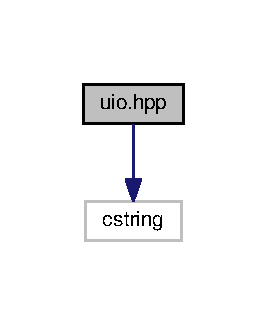
\includegraphics[width=128pt]{uio_8hpp__incl}
\end{center}
\end{figure}
\subsection*{Classes}
\begin{DoxyCompactItemize}
\item 
class \hyperlink{classuio_1_1streamerr}{uio\+::streamerr}
\begin{DoxyCompactList}\small\item\em Class to manage stream errors. \end{DoxyCompactList}\item 
class \hyperlink{classuio_1_1stream__base}{uio\+::stream\+\_\+base}
\begin{DoxyCompactList}\small\item\em Base class for all stream objects. \end{DoxyCompactList}\item 
class \hyperlink{classuio_1_1streambuf}{uio\+::streambuf}
\begin{DoxyCompactList}\small\item\em A simple byte-\/buffer. \end{DoxyCompactList}\item 
class \hyperlink{classuio_1_1istream}{uio\+::istream}
\begin{DoxyCompactList}\small\item\em An input data object. \end{DoxyCompactList}\item 
class \hyperlink{classuio_1_1ostream}{uio\+::ostream}
\begin{DoxyCompactList}\small\item\em An output data object. \end{DoxyCompactList}\item 
class \hyperlink{classuio_1_1iostream}{uio\+::iostream}
\begin{DoxyCompactList}\small\item\em An input and output data stream. \end{DoxyCompactList}\end{DoxyCompactItemize}


\subsection{Detailed Description}
\begin{DoxyAuthor}{Author}
Liam Bindle \href{mailto:liam.bindle@usask.ca}{\tt liam.\+bindle@usask.\+ca} 
\end{DoxyAuthor}
\begin{DoxyVersion}{Version}
0.\+0 
\end{DoxyVersion}

%--- End generated contents ---

% Index
\backmatter
\newpage
\phantomsection
\clearemptydoublepage
\addcontentsline{toc}{chapter}{Index}
\printindex

\end{document}
